\chapter{Getting started with Dresden OCL}
\label{chapter:introduction}

\begin{flushright}
\textit{Chapter written by Claas Wilke and Michael Thiele}
\end{flushright}

This chapter generally introduces into \keyword{Dresden OCL}. Dresden OCL is
based on a \keyword{Pivot Model} developed by Matthias 
Br�uer~\cite{GB:Braeuer} which is shortly explained in 
Chapter~\ref{chapter:architecture}. Further information about Dresden OCL is 
available at the project's website~\cite{WWW:toolkit}.

This chapter explains the installation of Dresden OCL and how to load a 
model, an instance of such a model, and \acs{OCL} constraints defined on such a 
model into Dresden OCL. Besides the Eclipse distribution, Dresden OCL can 
also be used as a stand-alone Java Library. If you plan to use the stand-alone 
distribution you can skip this chapter and continue with 
Chapter~\ref{chapter:standalone}. However, this chapter explains the basic 
concepts of Dresden OCL. Although you cannot use the shown GUI wizards and 
browsers when using the stand-alone version, this chapter can be helpful to 
understand the terms used in and the mechanisms provided by Dresden OCL.
  


\section{How to Install Dresden OCL}
	
The following different possibilities exist to install Dresden OCL within
Eclipse.

\begin{enumerate}
	\item You may install Dresden OCL using the \emph{Eclipse Marketplace
	  Client}.
	\item You may install Dresden using the update site available
	  at~\cite{WWW:toolkitUpdatesite},
	\item You may checkout and run the source code distribution from the \acs{SVN}
	  available at~\cite{WWW:toolkitSVN}.
\end{enumerate}

This section will explain all three possibilities.
	

\subsection{Installing Dresden OCL using the Eclipse Marketplace Client}

Since Eclipse 3.6, the new Eclipse Marketplace Client allows easy installation
of Eclipse-based tools such as Dresden OCL.

To install Dresden OCL via the Eclipse Marketplace Client, select the menu
option \emph{Help -> Eclipse Marketplace\ldots}. Probably you have to select a
marketplace catalog afterwards. If so, select the \emph{Eclipse Marketplace}
catalog and proceed.

Type \texttt{Dresden OCL} into the search text field and press the return key.
Select Dresden OCL from the search results and click the \emph{Install} button
(cf. Fig.~\ref{pic:intro:marketplace01}). Afterwards, click through the
installation dialog and Dresden OCL will be installed. Finally you have to 
restart your Eclipse distribution to complete the installation.

\begin{figure}[!b]
	\centering
	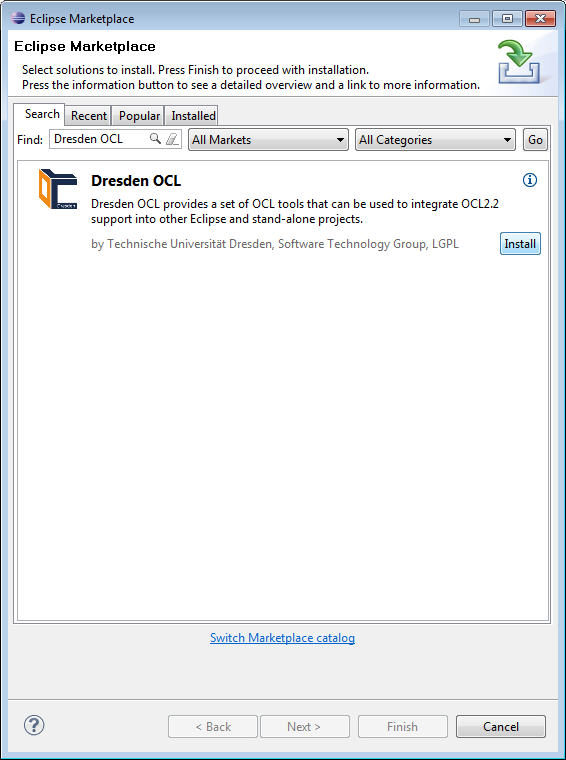
\includegraphics[width=0.8\linewidth]{figures/introduction/marketplace01}
	\caption{Installing Dresden OCL using the Marketplace Client.}
	\label{pic:intro:marketplace01}
\end{figure}


\subsection{Installing Dresden OCL using the Eclipse Update Site}
	
To install Dresden OCL via the \keyword{Eclipse Update Site}, you have to
start an Eclipse instance and select the menu option \eclipse{Help ->
Install New Software\ldots}

Enter the path \url{http://dresden-ocl.sourceforge.net/downloads/updatesite/site.xml} 
and click the \eclipse{Add...} button (cf. Fig.~\ref{pic:intro:updateSite01}).
In the new opened window you can additionaly enter a name for the update site 
(cf. Fig.~\ref{pic:intro:updateSite02}).

\begin{figure}[!b]
	\centering
	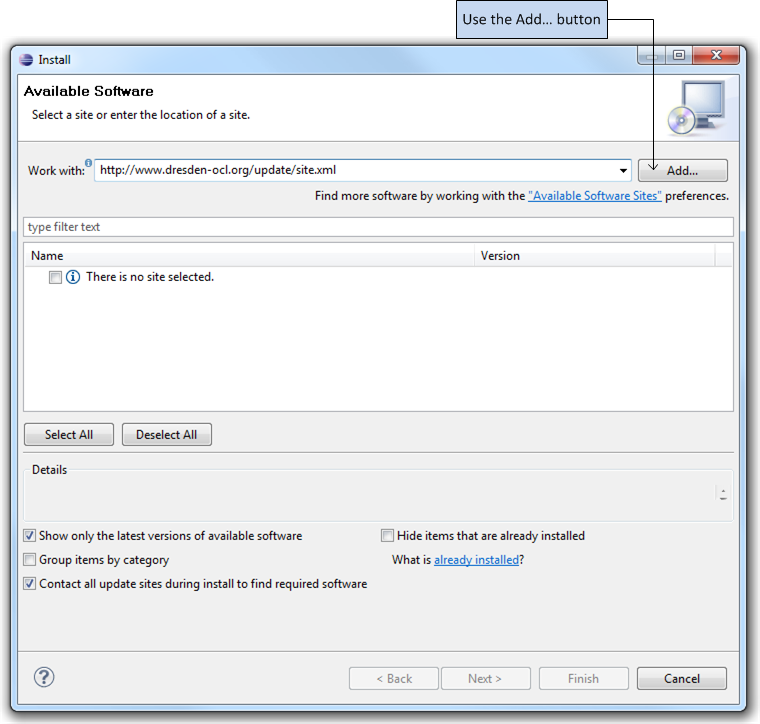
\includegraphics[width=0.8\linewidth]{figures/introduction/updateSite01}
	\caption{Adding an Eclipse Update Site (Step 1).}
	\label{pic:intro:updateSite01}

  \vspace{2.0em}
  
	\centering
	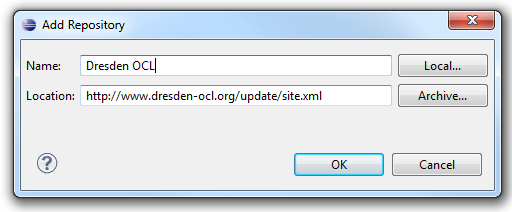
\includegraphics[width=0.6\linewidth]{figures/introduction/updateSite02}
	\caption{Adding an Eclipse Update Site (Step 2).}
	\label{pic:intro:updateSite02}
\end{figure}

Now you can select the features of Dresden OCL which you want to install. 
Select them and click the \eclipse{Next >} button (cf. 
Fig.~\ref{pic:intro:updateSite03}). An overview on all features of 
Dresden OCL can be found in Table~\ref{tab:plugins} in the appendix of 
this manual. Follow the wizard and agree with the user license. Then Dresden OCL
will be installed. Afterwards, you should restart your Eclipse application to 
finish the installation.

\begin{figure}[t]
	\centering
	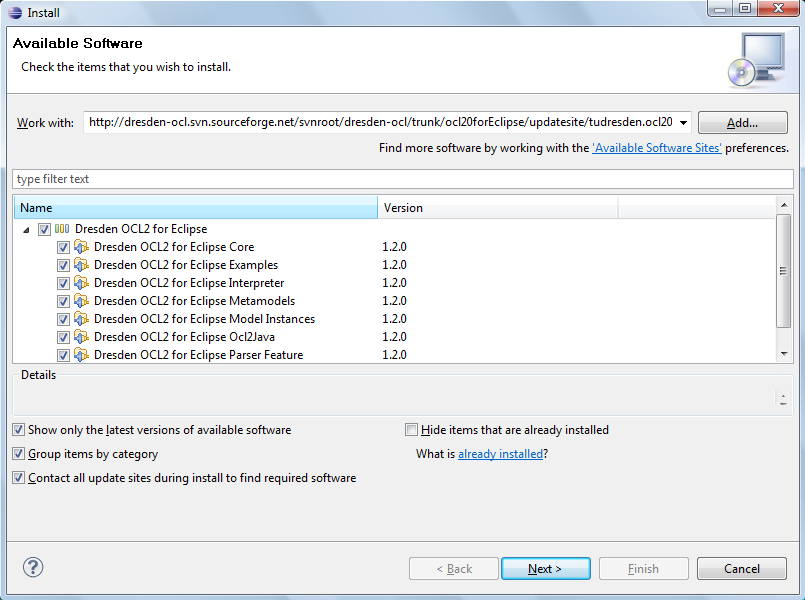
\includegraphics[width=1.0\linewidth]{figures/introduction/updateSite03}
	\caption{Selecting features of Dresden OCL.}
	\label{pic:intro:updateSite03}
\end{figure}
	
	
\subsection{Importing Dresden OCL from the SVN}

To use Dresden OCL by checking out the source code from the \acs{SVN} you
need to install an \acs{SVN} client. In the following the 
\keyword{Eclipse Subversive} plug-in is used.

After installing Eclipse Subversive, a new \keyword{Eclispe Perspective} 
providing access to \acs{SVN} should exist. The perspective can be opened via 
the menu \eclipse{Window > Open Perpective > Other... > SVN Repository
Exploring}. In the view \eclipse{\acs{SVN} Repositories} you can add a new 
repository using the \acs{URL} 
\url{https://dresden-ocl.svn.sourceforge.net/svnroot/dresden-ocl/} (cf. 
Fig.~\ref{pic:intro:svn01}).

\begin{figure}[!b]
	\centering
	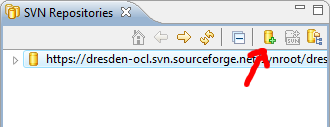
\includegraphics[width=0.5\linewidth]{figures/introduction/svn01}
	\caption{Adding an SVN repository.}
	\label{pic:intro:svn01}
\end{figure}

After clicking the \eclipse{Finish} button, the \acs{SVN} repository root should 
be visible in the \eclipse{\acs{SVN} Repositories} view. To checkout the
plug-ins, you have to select them in the repository directory 
\reference{trunk/ocl20\-for\-Eclipse/eclipse} and use the \eclipse{Checkout...} 
function in the context menu (cf. Fig.~\ref{pic:intro:svn02}).
	
\begin{figure}[!t]
	\centering
	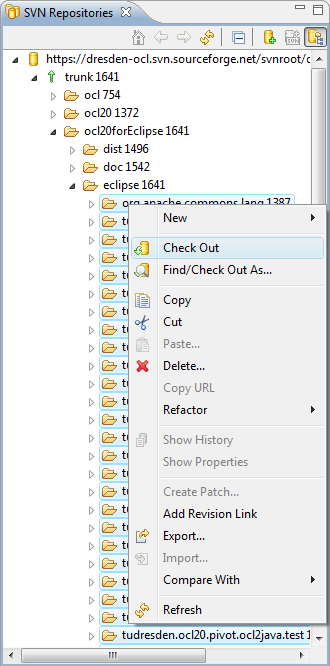
\includegraphics[width=0.5\linewidth]{figures/introduction/svn02}
	\caption{Checkout of Dresden OCL's plug-in projects.}
	\label{pic:intro:svn02}
\end{figure}


\subsection{Which Plug-ins do you need at least?}

Often people wonder which plug-ins of Dresden OCL they require for a
minimum installation. The answer to this question depends on the things you 
plan to do with Dresden OCL. Table~\ref{tab:plugins} in the appendix of 
this manual shows a list of the currently existing plug-ins of
Dresden OCL, that are related to different features. You should install 
at least the \keyword{Core} feature, at least one meta-model of the 
\keyword{Meta-Models} feature, and the complete \keyword{Parser} feature. The 
\keyword{Interpreter}, the \keyword{OCL22Java}m and the
\keyword{OCL2SQL} features are only required if you want to interpret
constraints or to generate code from constraints, respectively. If you import or interpret model instances, you need to install 
the \keyword{Model Instances} feature as well. The examples of the 
\keyword{Example} feature are only required to run the examples provided in 
this manual. We recommend to install all provided features.
		

\subsection{Building the OCL2 Parser}
The new Dresden OCL parser/editor is partially written in Scala. In order
to build the sources of the parser without having to have the \reference{Scala
IDE} installed, Dresden OCL comes with various \keyword{Ant} scripts that
compile the Scala code to byte code.

After a checkout, the build script should be called automatically. Be aware that
the compilation might take a while to finish. If other projects that depend on
the parser like the facade still do not compile correctly, try to perform a 
\keyword{refresh} on the plug-ins that contain Scala code.

If the \keyword{Ant} script is not invoked automatically, you can call it either
be cleaning the
\reference{tudresden\linebreak[0].ocl\-20\linebreak[0].pivot.language.ocl.staticsemantics}
plug-in or by running the \keyword{Ant} task \reference{clean all} of the same plug-in.

Each plug-in that contains Scala code (\reference{org.kiama.attribution},
\reference{tudresden.ocl20.pivot\linebreak[0].lan\-guage\linebreak[0].ocl.semantics},
\reference{tudresden.ocl20.pivot.language.ocl.staticsemantics} and
\reference{tu\-dres\-den\linebreak[0].ocl20.pivot.pivotmodel.semantics})
contains a
\keyword{build.xml} file that comes with three targets: \reference{clean all}
to clean the selected project and all dependent projects, \reference{clean} to
only clean the selected project and \reference{compile} to simply compile changes
that have been made since the last build.

In either case, you have to run the \keyword{ANT} scripts in the same 
\keyword{JRE} as Eclipse. Figures~\ref{pic:intro:parserbuild01} 
and~\ref{pic:intro:parserbuild02} show how to achieve this. If an error like 
``Unable to find javac compiler.'' occurs, you might be trying to run the
\keyword{Ant} script with a \keyword{\acl{JRE}} instead of a \keyword{\acs{JDK}}
(For errors like this one) use the \eclipse{Installed JREs...} button in the
same window to select a \acs{JDK} instead.

If you want to make changes to the static semantics evaluation of the parser you
should consider installing the \emph{Scala IDE} from 
\url{http://www.scala-lang.org/scala-eclipse-plugin}. Be aware that the Scala
code is version 2.7.7 which is not compatible with Scala 2.8 and therefore you
cannot use the current \emph{Scala IDE} which supports only Scala 2.8. The
\emph{Scala IDE} runs with Eclipse 3.5 and 3.6.

In order to use the Scala compiler of the IDE, you have to go to the
\eclipse{Properties} of each Scala plug-in, select the tab \eclipse{Builders},
check the \eclipse{Scala Builder} and possibly uncheck the \keyword{Ant} script
for building.

\begin{figure}[p]
	\centering
	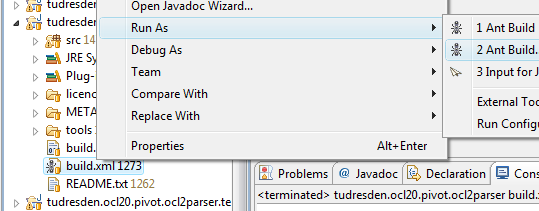
\includegraphics[width=0.8\linewidth]{figures/introduction/parserbuild01}
	\caption{Executing the OCL2 Parser build script.}
	\label{pic:intro:parserbuild01}

  \vspace{4.0em}

	\centering
	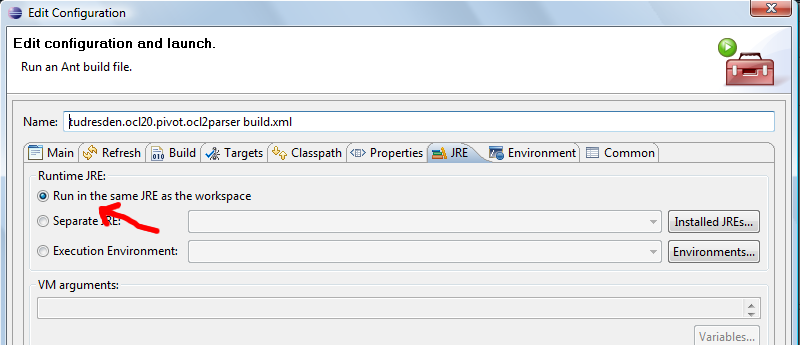
\includegraphics[width=0.8\linewidth]{figures/introduction/parserbuild02}
	\caption{Settings of the JRE for the Ant build script.}
	\label{pic:intro:parserbuild02}

  \vspace{4.0em}

	\centering
	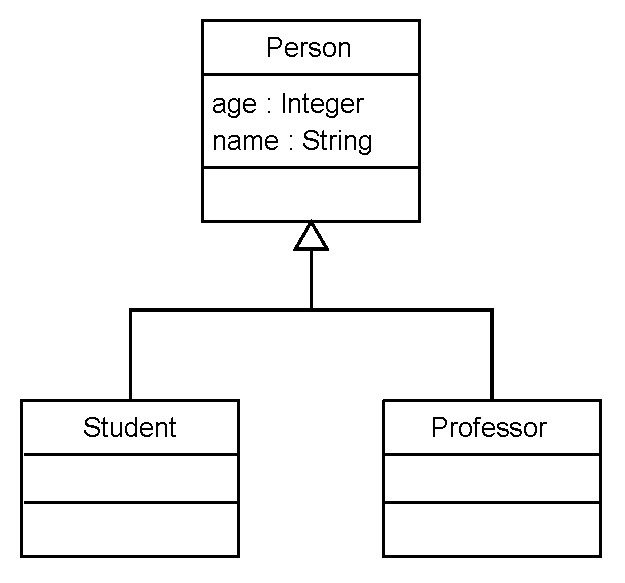
\includegraphics[width=0.5\linewidth]{figures/examples/simple01}
	\caption{A class diagram describing the Simple Example model.}
	\label{pic:examples:simple01}
\end{figure}


\section{Loading Models, Model Instances and Constraints}

If you installed the Dresden OCL using the market place client or update site,
you can execute the toolkit within your Eclipse distribution. If you imported
the Toolkit as source code plug-ins into an Eclipse workspace, you have to start a 
new Eclipse instance. You can start a new instance via the menu \eclipse{Run >
Run As > Eclipse Application}. If the menu \eclipse{Eclipse Application} is not 
available or disabled you need to select one of the plug-ins of the toolkit in
the \eclipse{Package Explorer} first.


\subsection{The Simple Example}
\label{intro:simpleExample}

The use of Dresden OCL is explained using the \keyword{Simple Example} 
which is located in the plug-in 
\reference{tudresden.ocl20.pivot.examples.\linebreak[0]simple}. 
Figure~\ref{pic:examples:simple01} shows a class diagram of the Simple Example.

Dresden OCL provides more examples than the Simple Example. The different 
examples use different meta-models which is possible with the \textit{Pivot
Model} architecture of the Toolkit. An overview about all examples provided 
with Dresden OCL is listed in Table~\ref{tab:examples} in the appendix of
this manual. The Simple Example can be used with two different meta-models. 
These are \keyword{\acs{UML} 2} (based on \keyword{\acs{Eclipse MDT} 
\acs{UML}}) and \keyword{Java}.


\subsection{Dresden OCL Perspective}

Dresden OCL provides its own perspective within Eclipse that contains all views
and editors provided with Dresden OCL. To ease the work with Dresden OCL, you
should now switch to the Dresden OCL perspective. Select the menu option
\eclipse{Window -> Open Perspective -> Other \ldots} and select the perspective
\eclipse{Dresden OCL} (cf. Fig.~\ref{pic:introduction:perspective})
	
\begin{figure}[!t]
	\centering
	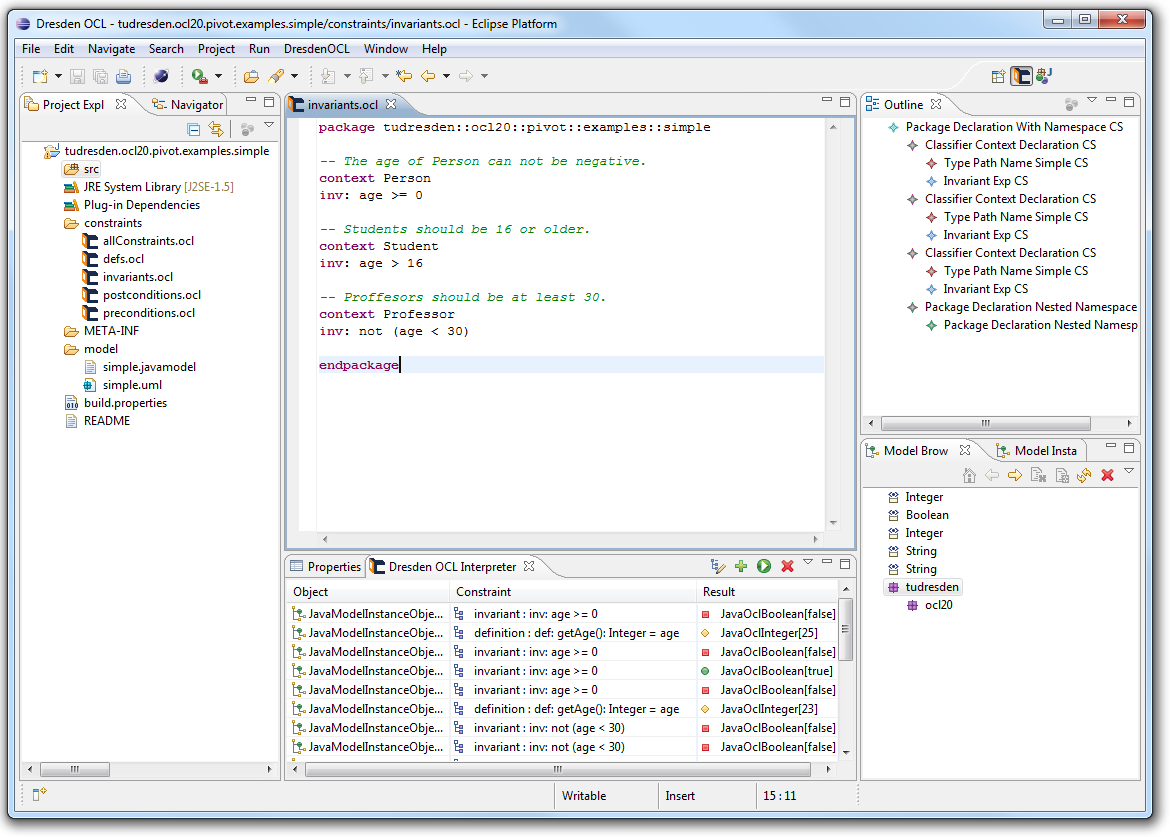
\includegraphics[width=1.0\linewidth]{figures/introduction/perspective}
	\caption{The Dresden OCL Perspective.}
	\label{pic:introduction:perspective}
\end{figure}

On the left hand side the perspective contains the \eclipse{Project Explorer} of
Eclipse to manage different projects. The right hand side contains the
\eclipse{Outline View} for opened \acs{OCL} files. Below, the \eclipse{Model
Browser} and \eclipse{Model Instance Browser} of Dresden OCL allow to explore models and
instances imported into Dresden OCL. At the bottom of the perspective the
\eclipse{OCL Intepreter} is located. The center of the perspective contains the
\eclipse{OCL Editor} of Dresden OCL that allows to edit and parse \acs{OCL}
files for an opened model. How to use the tools provided with Dresden OCL is explained in
the following.


\subsection{Loading a Model}
	
For this tutorial you first have to load a model into Dresden OCL. To ease the
use of the Simple Example project, this project should be imported into the  
\keyword{Workspace} first. Select the menu option \emph{File -> New ->
Other} and select the option \emph{Dresden OCL Examples -> Simple Example}
within the new opened window (cf. Fig~\ref{pic:intro:importexample01}). Click
the \emph{Finish} button to import the project into your workspace. Afterwards, the workspace should contain the Simple
Example project as shown in Figure~\ref{pic:introduction:perspective}, left hand
side.

\begin{figure}[!t]
	\centering
	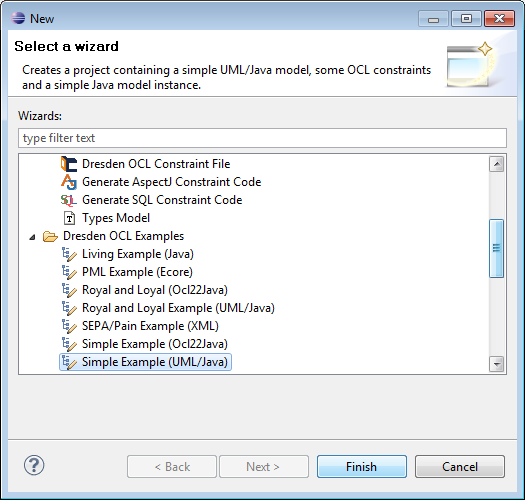
\includegraphics[width=0.8\linewidth]{figures/introduction/importexample01}
	\caption{Importing the Simple Example project.}
	\label{pic:intro:importexample01}
\end{figure}

Now you can import the model into Dresden OCL. Select the
\reference{model/simple.uml} file in the \eclipse{Project Explorer} and open the
context menu (right mouse click). Select the menu option
\eclipse{Dresden OCL > Load Model} (cf. Fig.~\ref{pic:intro:loadmodel00}). In
the opened wizard you have to select the meta-model \acs{UML}2 and click the
\eclipse{Finish} button (cf. Fig.~\ref{pic:intro:loadmodel01}).

Figure~\ref{pic:intro:loadmodel02} shows the imported Simple Example model,
which uses \acs{UML}2 as its meta-model. Via the menu button of the \eclipse{Model 
Browser} (the little triangle in the right top corner) you can switch between 
different models imported into Dresden OCL (cf.  
Fig.~\ref{pic:intro:loadmodel03}). With the two circled arrows icon you can
reload a model into Dresden OCL, with the red \emph{X} you can close the
currently selected model.
	
\begin{figure}[!p]
	\centering
	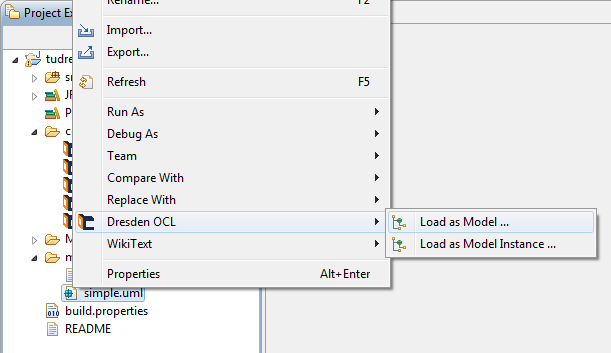
\includegraphics[width=1.0\linewidth]{figures/introduction/loadmodel00}
	\caption{Loading a Model.}
	\label{pic:intro:loadmodel00}
	
  \vspace{6.0em}
	\centering
	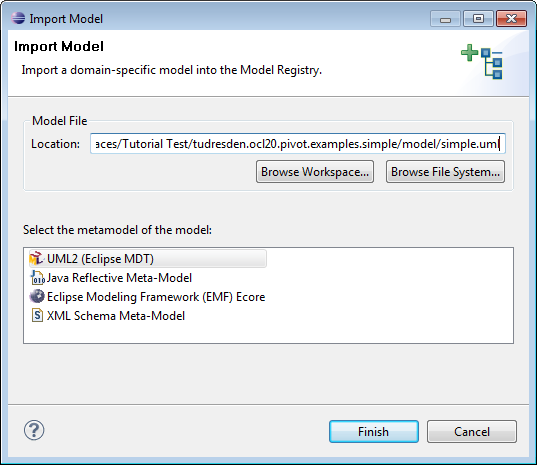
\includegraphics[width=0.7\linewidth]{figures/introduction/loadmodel01}
	\caption{Loading a Model.}
	\label{pic:intro:loadmodel01}
\end{figure}
	
\begin{figure}[!p]
	\centering
	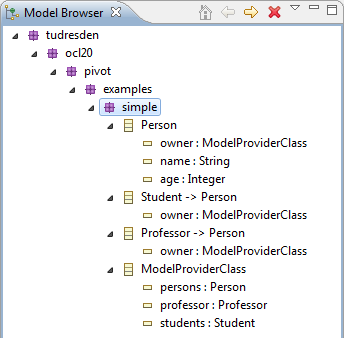
\includegraphics[width=0.4\linewidth]{figures/introduction/loadmodel02}
	\caption{The Simple Example model within the Model Browser.}
	\label{pic:intro:loadmodel02}
	
	\vspace{6.0em}

	\centering
	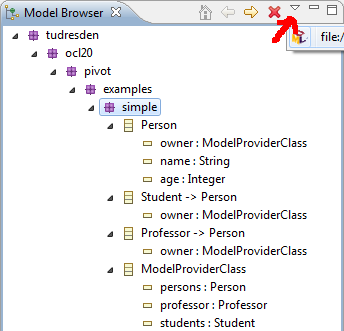
\includegraphics[width=0.4\linewidth]{figures/introduction/loadmodel03}
	\caption{You can switch between different Models using the little triangle.}
	\label{pic:intro:loadmodel03}
	
\end{figure}

	
\subsection{Loading a Model Instance}
\label{intro:loadModel}

After loading a model, you can load an instance of this model using another 
wizard. The model instance is required to interpret \acs{OCL} constraints on
elements instantiating the classes described in the opened model. Which kinds
of model instances are supported in Dresden OCL is documented in
Section~\ref{sect:info:modelinstances}. 
Since the Simple Example provides a Java model instance, we now have to select a
\code{class} file. \code{class} files are not displayed in the \eclipse{Project
Explorer}. Thus, switch to the \eclipse{Navigator} that should be visible at the
left hand side of the Dresden OCL perspective as well and select the
file
\reference{bin/tudresden/ocl20/\linebreak[0]pivot/examples/\linebreak[0]sim\-ple/\linebreak[0]in\-stance/\linebreak[0]Mo\-del\-InstanceProviderClass\linebreak[0].class}
of the Simple Example in the \eclipse{Project Explorer}. Open the context menu 
and select the menu option \eclipse{Dresden OCL > Load Model Instance} (cf.
Fig.~\ref{pic:intro:loadInstance00}).
In the opened wizard you have to select a model for which the model instance 
shall be loaded and the type of model instance you want to load (cf.
Fig.~\ref{pic:intro:loadInstance01}). Select the \keyword{Java Instance} type
and click the \eclipse{Finish} button.

\begin{figure}[!p]
	\centering
	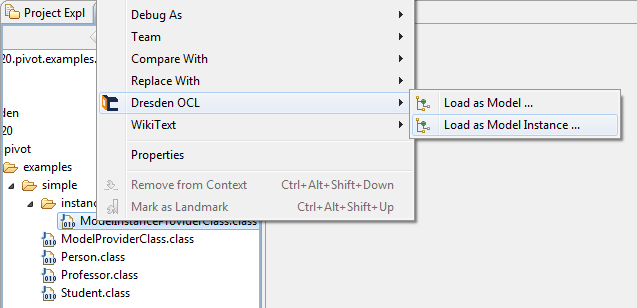
\includegraphics[width=0.7\linewidth]{figures/introduction/loadinstance00}
	\caption{Loading a Simple Model Instance.}
	\label{pic:intro:loadInstance00}

  	\vspace{6.0em}
  
	\centering
	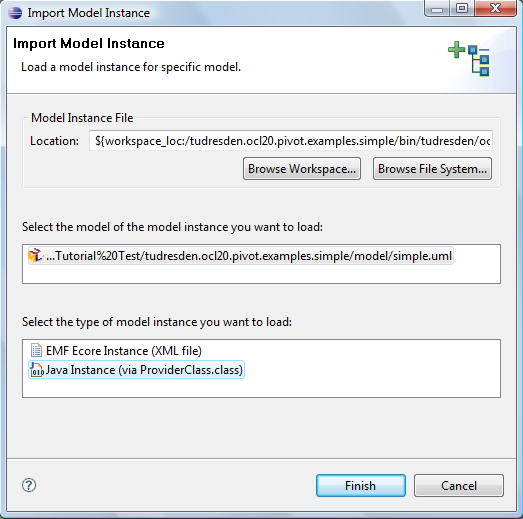
\includegraphics[width=0.7\linewidth]{figures/introduction/loadinstance01}
	\caption{Loading a Simple Model Instance.}
	\label{pic:intro:loadInstance01}
\end{figure}

Figure~\ref{pic:intro:loadInstance02} shows the imported model instance. Like
in the model browser you can switch between different model instances and you 
can close selected instances. Note that the \eclipse{Model Instance Browser} 
only shows the model instances of the model actually selected in the model 
browser. By switching the model in the model browser, you also switch the pool 
of model instances available in the model instance browser.

\begin{figure}[!p]
	\centering
	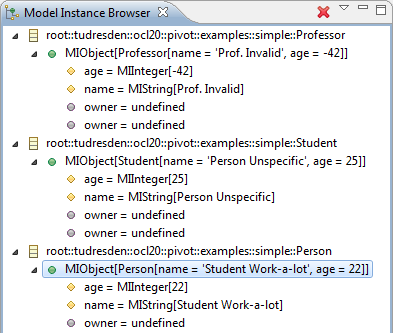
\includegraphics[width=0.6\linewidth]{figures/introduction/loadinstance02}
	\caption{A simple model instance in the Model Instance Browser.}
	\label{pic:intro:loadInstance02}

	\vspace{4.0em}
	
	\centering
	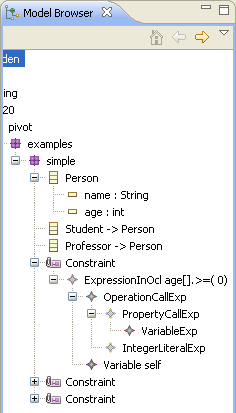
\includegraphics[width=0.4\linewidth]{figures/introduction/loadconstraints02}
	\caption{Parsed expressions and the model in the Model Browser.}
	\label{pic:intro:loadconstraints02}
\end{figure}
	
	
\subsection{Parsing OCL Expressions}
\label{intro:oclEditor}
Any file with the file extension \texttt{.ocl} can be opened with the
\keyword{Dresden OCL Editor}. Once opened, syntactic checks are performed
to analyse whether the given file contains valid \acs{OCL} code. If currently
there is no active model selected in the \eclipse{Model Browser}, the editor
will fail to perform the static semantics analysis and will yield that there is
no active model. You can load a model and then re-parse the \acs{OCL} file by
changing the \acs{OCL} file (e.g., by introducing and immediately deleting a
whitespace character).

The editor/parser will automatically add parsed constraints to the
model as well as \keyword{definitions} to the appropriate
classes. You can inspect the changes on the model in the \eclipse{Model
Browser}. Note that the \keyword{definitions} and constraints are not added to
your model -- they belong to the view of Dresden OCL on the model. The result
can be seen in Figure~\ref{pic:intro:loadconstraints02}. You also can remove
parsed constraints from the model which is shown in
Figure~\ref{pic:intro:loadconstraints03}.

\begin{figure}[t]
	\centering
	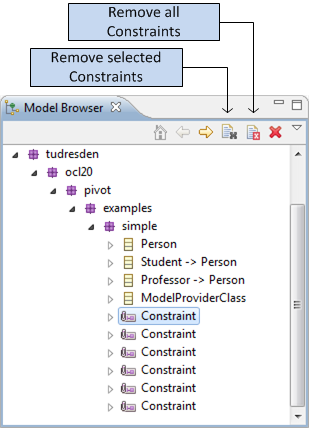
\includegraphics[width=0.4\linewidth]{figures/introduction/loadconstraints03}
	\caption{How to remove Constraints from a Model again.}
	\label{pic:intro:loadconstraints03}
\end{figure}

	

\section{Summary}
  
This chapter described how to use Dresden OCL. It was explained how to 
install the plug-ins of Dresden OCL. Afterwards, the import of models,
model instances and \acs{OCL} constraints into Dresden OCL was explained.

Now, the imported models can be used with the tools provided by Dresden OCL. For
example you can use the \keyword{OCL Interpreter} to interpret \acs{OCL} 
constraints for a given model and model instance (as explained in 
Chapter~\ref{chapter:interpretation}) or you can use the \keyword{OCL22Java
Code Generator} to generate \keyword{AspectJ} code for a loaded model and 
\acs{OCL} constraints (as explained in Chapter~\ref{chapter:codeGeneration}).
How the \keyword{OCL2SQL Code Generator} can be used to generated SQL schema and
integretiy views is documented in Chapter~\ref{chapter:ocl2sql}.

If you do not want to use Eclipse, but still want to interpret OCL constraints 
or generate AspectJ code, you can use Dresden OCL as a stand-alone library
outside of Eclipse. A detailed description on how to do this is given in 
Chapter~\ref{chapter:standalone}.
